%%%%%%%%%%%%%%%%%%%%%%%%%%%%%%%%%%%%%%%%%%%%%%%%%%%%%%%%%%%%%%%%%%%%%%%%%%%%%%%%%%%
%% This project aims to create the UFC template for presentation.                %%
%% author: Maurício Moreira Neto - Doctoral student in Computer Science (MDCC)   %%
%% contacts:                                                                     %%
%%    e-mail: maumneto@ufc.br                                                    %%
%%    linktree: https://linktr.ee/maumneto                                       %%
%%%%%%%%%%%%%%%%%%%%%%%%%%%%%%%%%%%%%%%%%%%%%%%%%%%%%%%%%%%%%%%%%%%%%%%%%%%%%%%%%%%
\documentclass{libs/ufc_format}
% Inserting the preamble file with the packages
%%%%%%%%%%%%%%%%%%%%%%%%%%%%%%%%%%%%%%%%%%%%%%%%%%%%%%%%%%%%%%%%%%%%%
%% This file contains the packages that can be used in the beamer. %%
%%%%%%%%%%%%%%%%%%%%%%%%%%%%%%%%%%%%%%%%%%%%%%%%%%%%%%%%%%%%%%%%%%%%%
% Package to fonts family
\usepackage[T1]{fontenc}
% Package to accentuation
\usepackage[utf8]{inputenc}
% Package to Portuguese language
\usepackage[brazil]{babel}
% Package to Figures
\usepackage{graphicx}
% Package to the colors
\usepackage{color}
% Package to the colors
\usepackage{xcolor}
% Packages to math symbols and expressions
\usepackage{amsfonts, amssymb, amsmath}
% Package to multiple lines and columns in table
\usepackage{multirow, array} 
% Package to create pseudo-code
% For more detail of this package: http://linorg.usp.br/CTAN/macros/latex/contrib/algorithm2e/doc/algorithm2e.pdf
\usepackage{algorithm2e}
% Package to insert code
% \usepackage{listings} 
% \usepackage{keyval}
% Package to justify text
\usepackage[document]{ragged2e}
% Package to manage the bibliography
\usepackage[backend=biber, style=numeric, sorting=none]{biblatex}
% Package to facilities quotations
\usepackage{csquotes}
% Package to use multicols
\usepackage{multicol}
% Inserting the references file
\bibliography{references.bib}

% Title
\title[SOLID]{\huge\textbf{Princípios SOLID}}
% Subtitle
\subtitle{Aplicando os Princípios SOLID na Prática}
% Author of the presentation
\author{Gustavo Gurgel Medeiros}
\date{\today}


%%%%%%%%%%%%%%%%%%%%%%%%%%%%%%%%%%%%%%%%%%%%%%%%%%%%%%%%%%%%%%%%%%%%%%%%%%%%%%%%%%
%% Start Document of the Presentation                                           %%               
%%%%%%%%%%%%%%%%%%%%%%%%%%%%%%%%%%%%%%%%%%%%%%%%%%%%%%%%%%%%%%%%%%%%%%%%%%%%%%%%%%
\begin{document}
%% ---------------------------------------------------------------------------
% First frame (with tile, subtitle, ...)
\begin{frame}{}
    \maketitle
\end{frame}

%% ---------------------------------------------------------------------------
% This presentation is separated by sections and subsections
\section{Princípios SOLID}
\subsection{O que/quais são?}
\begin{frame}{O que são os Princípios SOLID}
    Os princípios SOLID são um conjunto de \textbf{cinco diretrizes} de design
    de software definidas por Robert C. Martin. O objetivo dessas diretrizes é
    ajudar a \textbf{criar sistemas mais compreensíveis, flexíveis e fáceis de
    manter.}

    \vspace{25px}

    \begin{itemize}
        \item S $\rightarrow$ Single Responsibility
        \item O $\rightarrow$ Open-Closed 
        \item L $\rightarrow$ Liskov Substitution
        \item I $\rightarrow$ Interface Segregation
        \item D $\rightarrow$ Dependency Inversion
    \end{itemize}
\end{frame}

%% ---------------------------------------------------------------------------
\begin{frame}{Single Responsibility}
    \centering
    \textbf{Uma \emph{classe} deve ter apenas uma única responsabilidade}
\end{frame}

\begin{frame}{Exemplo \textcolor{gred}{Ruim}}
    \begin{figure}
        \centering
        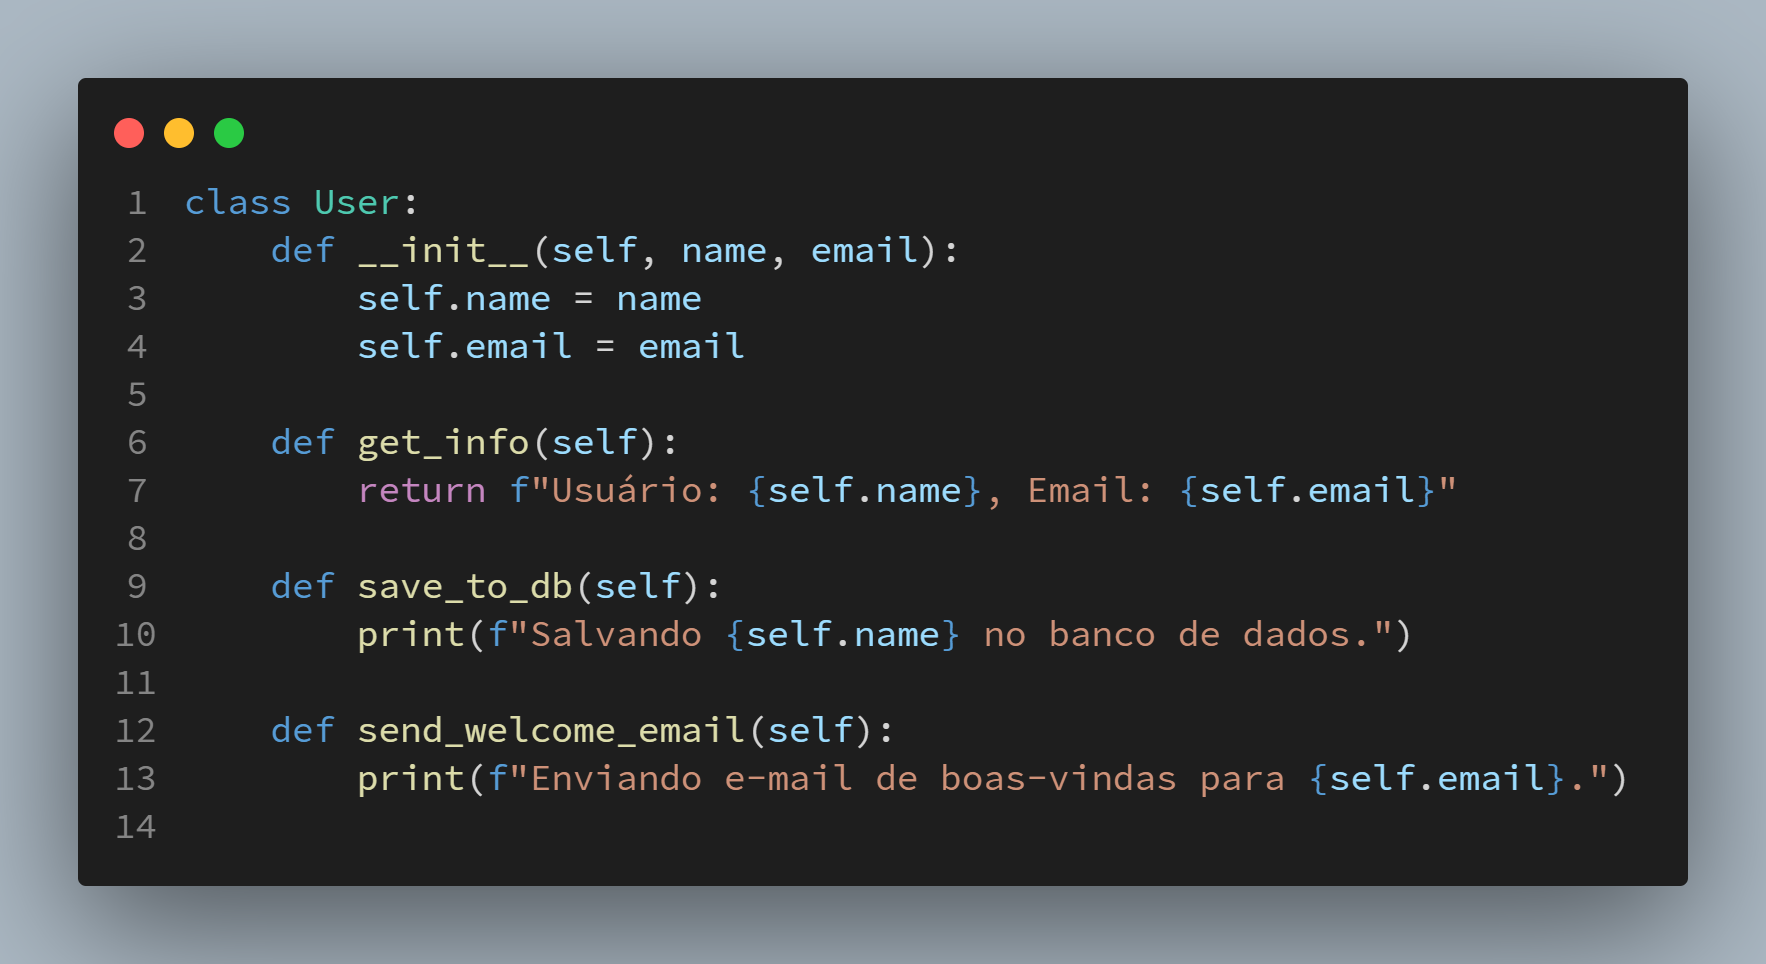
\includegraphics[scale=0.17]{images/s_exemple_bad.png}
    \end{figure}
\end{frame}

\begin{frame}{Exemplo \textcolor{ggreen}{Bom}}
    \begin{figure}
        \centering
        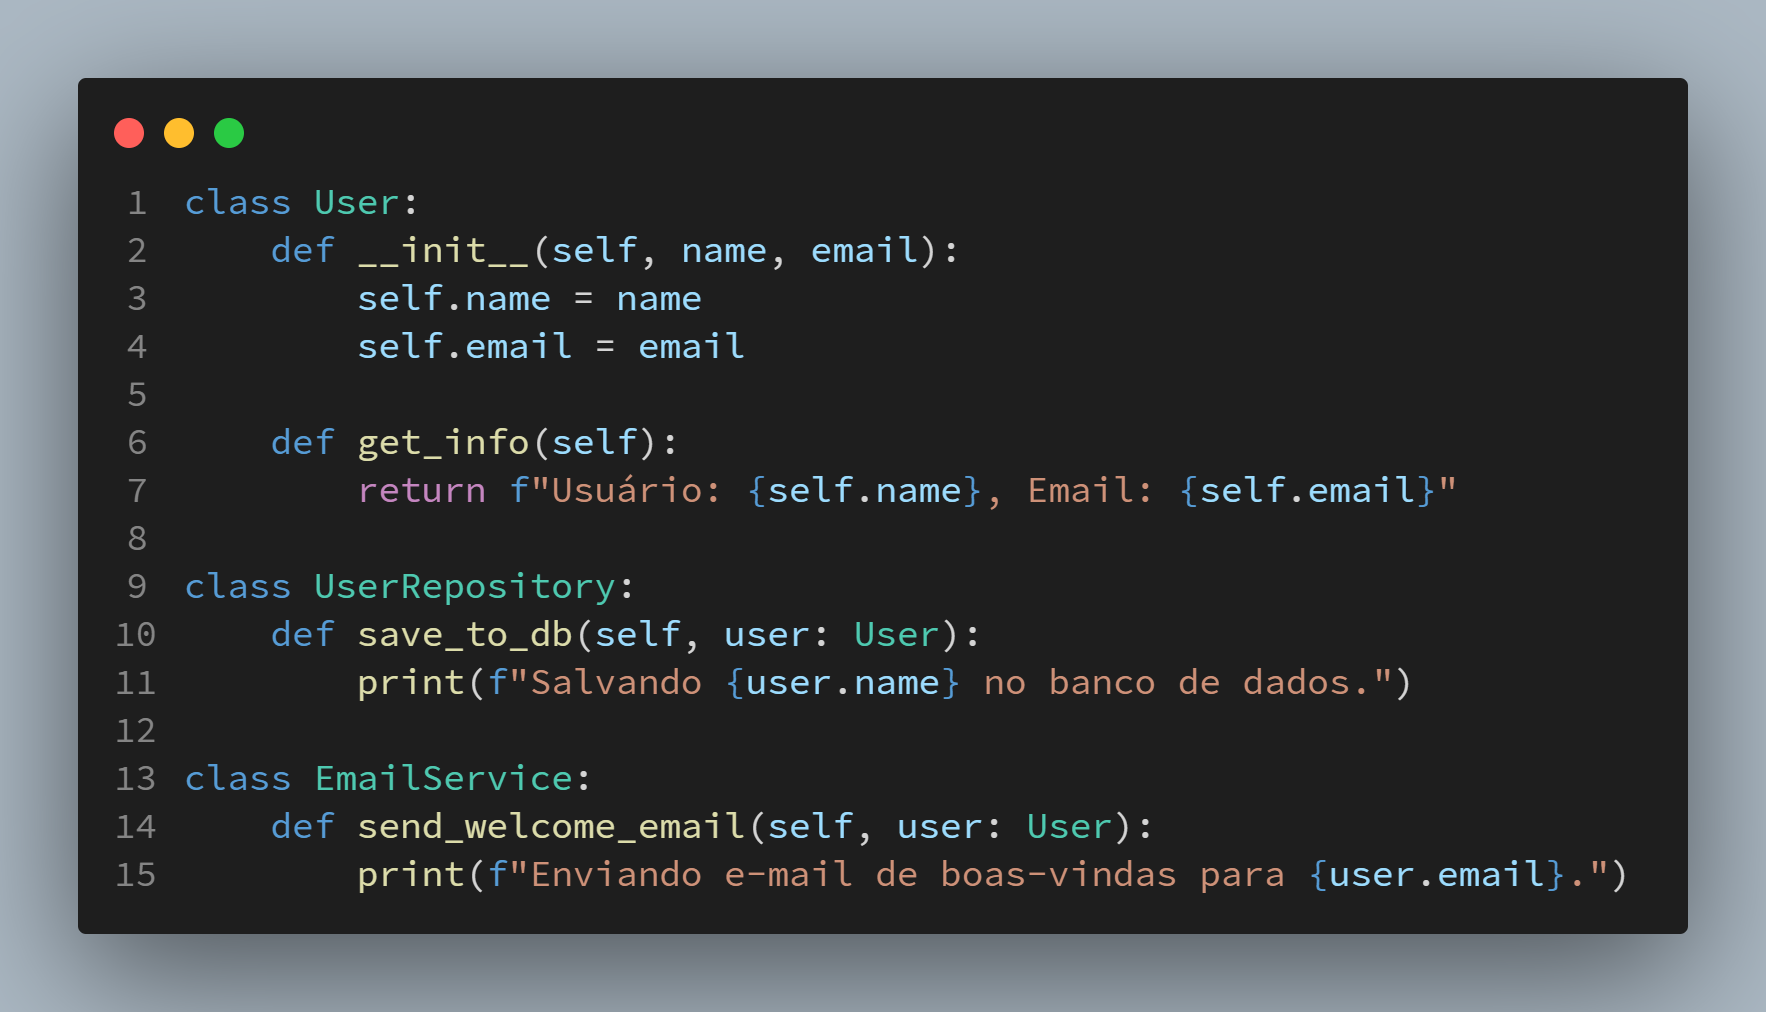
\includegraphics[scale=0.17]{images/s_example_good.png}
    \end{figure}
\end{frame}
%% ---------------------------------------------------------------------------

%% ---------------------------------------------------------------------------
\begin{frame}{Open-Closed}
    \centering
    \textbf{Uma \emph{classe} deve estar aberta para extensão, mas fechada para
    modificação.}
\end{frame}

\begin{frame}{Exemplo \textcolor{gred}{Ruim}}
    \begin{figure}
        \centering
        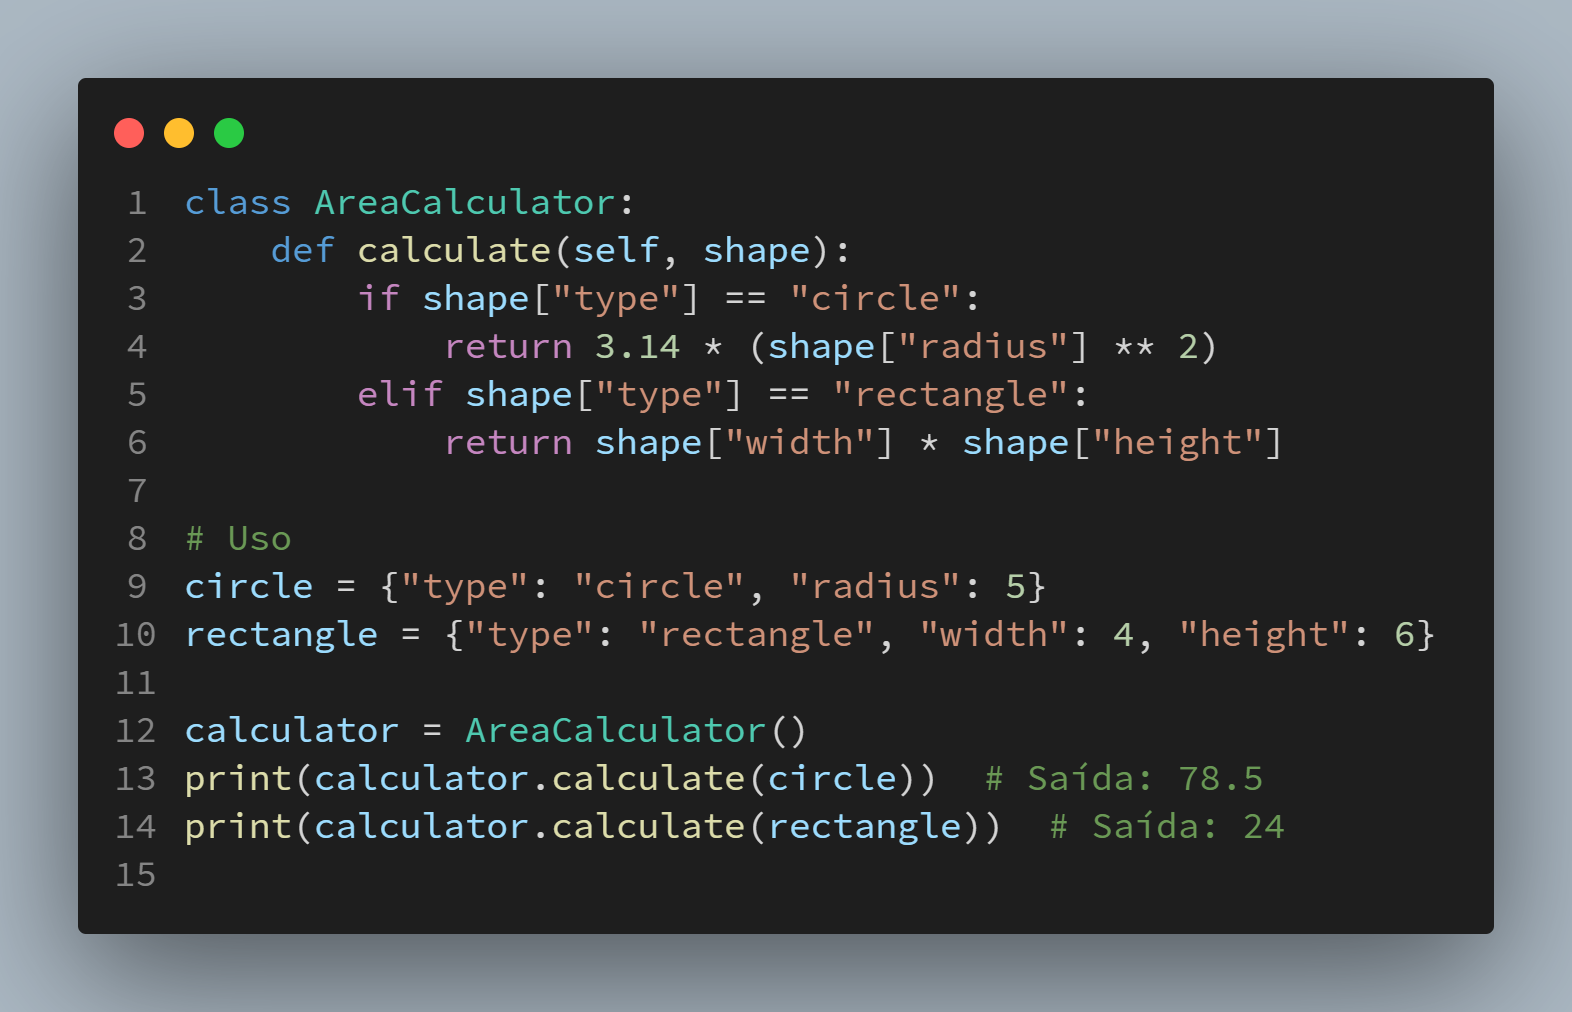
\includegraphics[scale=0.17]{images/o_exemple_bad.png}
    \end{figure}
\end{frame}

\begin{frame}{Exemplo \textcolor{ggreen}{Bom}}
    \begin{figure}
        \centering
        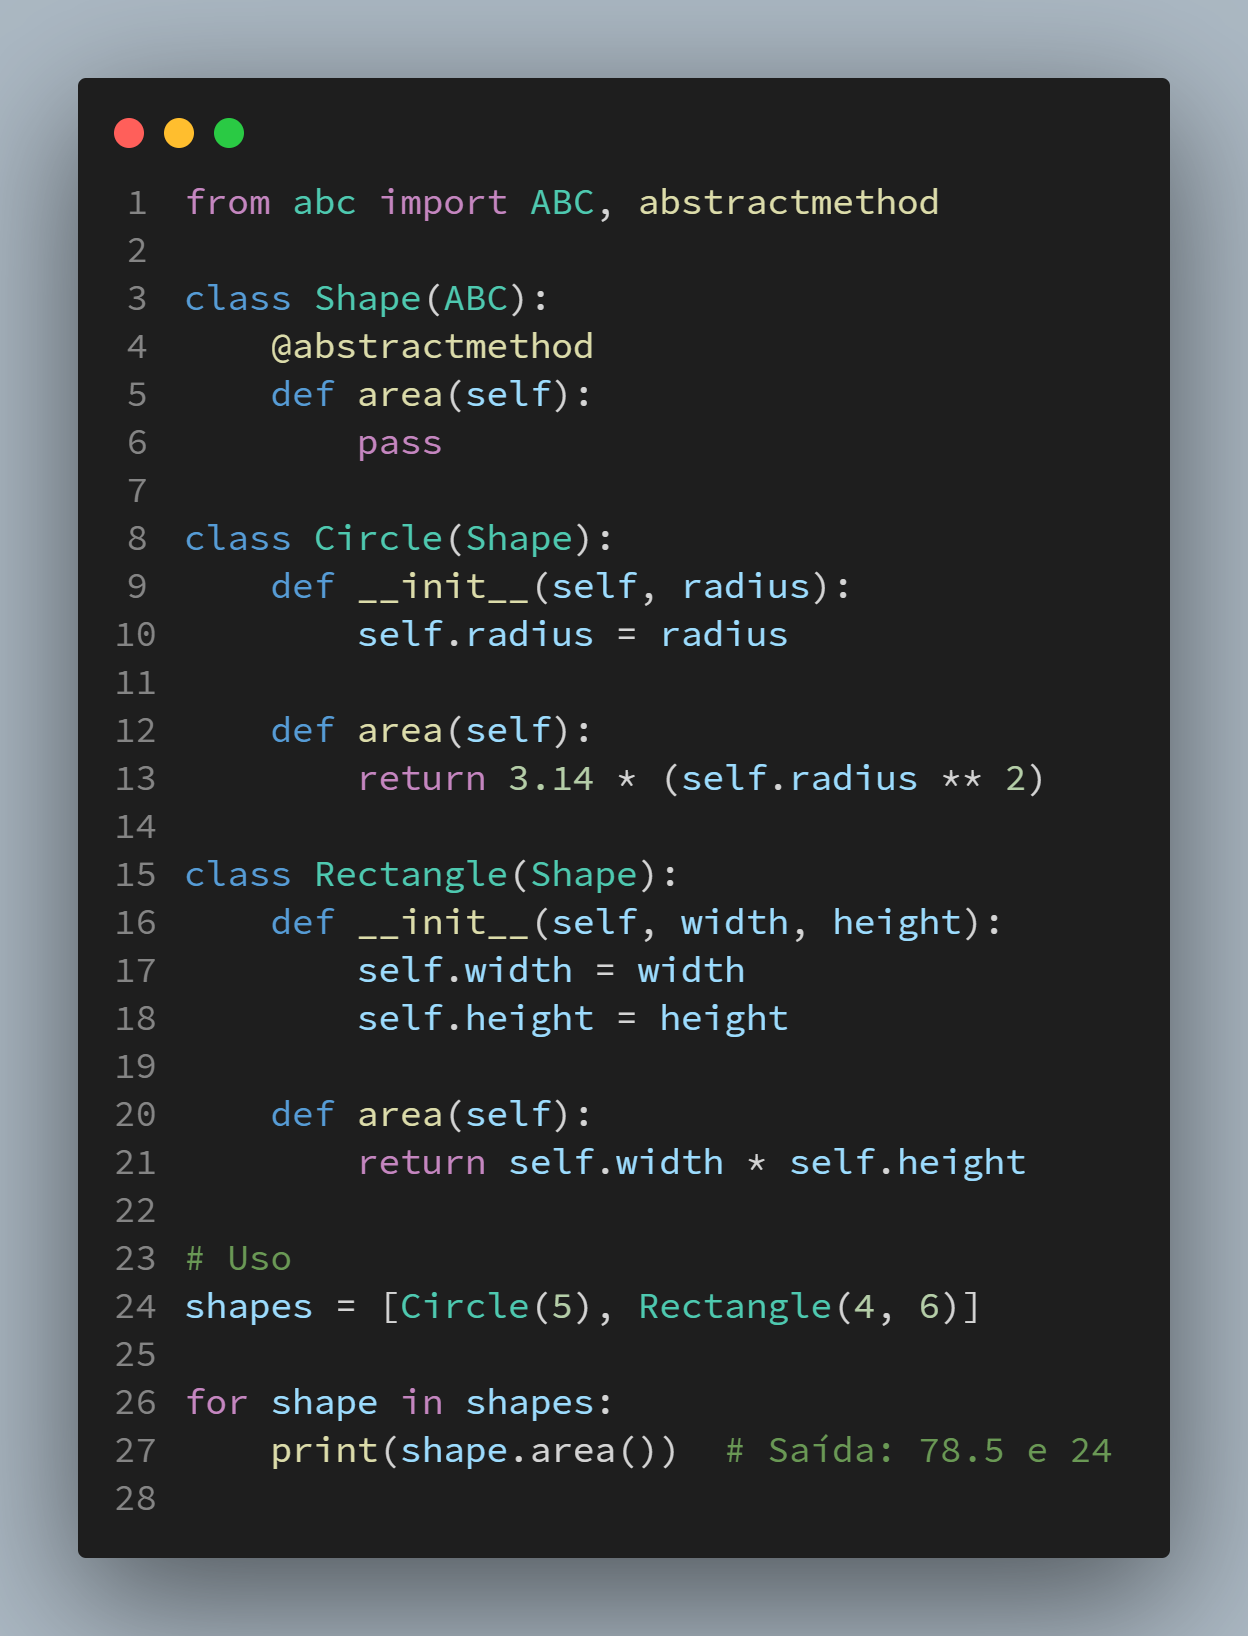
\includegraphics[scale=0.13]{images/o_exemple_good.png}
    \end{figure}
\end{frame}
%% ---------------------------------------------------------------------------

%% ---------------------------------------------------------------------------
\begin{frame}{Liskov Substitution}
    \centering
    \textbf{Uma \emph{subclasse} deve poder substituir sua \emph{superclasse}
     sem alterar o comportamento esperado.}
\end{frame}

\begin{frame}{Exemplo \textcolor{gred}{Ruim}}
    \begin{figure}
        \centering
        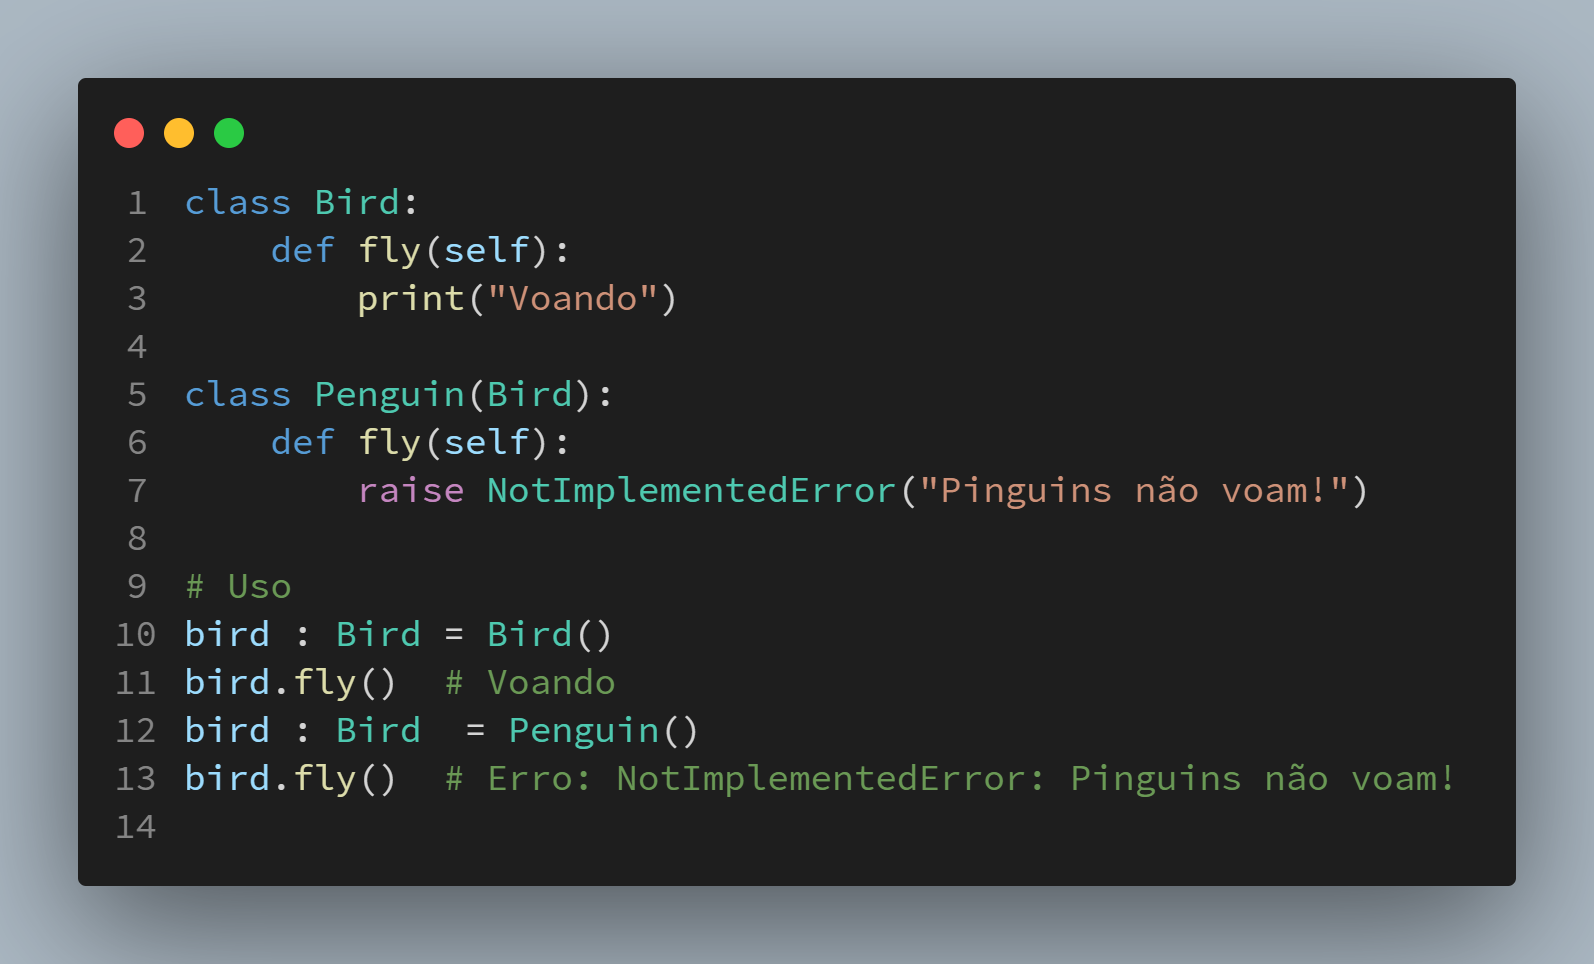
\includegraphics[scale=0.18]{images/l_exemple_bad.png}
    \end{figure}
\end{frame}

\begin{frame}{Exemplo \textcolor{ggreen}{Bom}}
    \begin{figure}
        \centering
        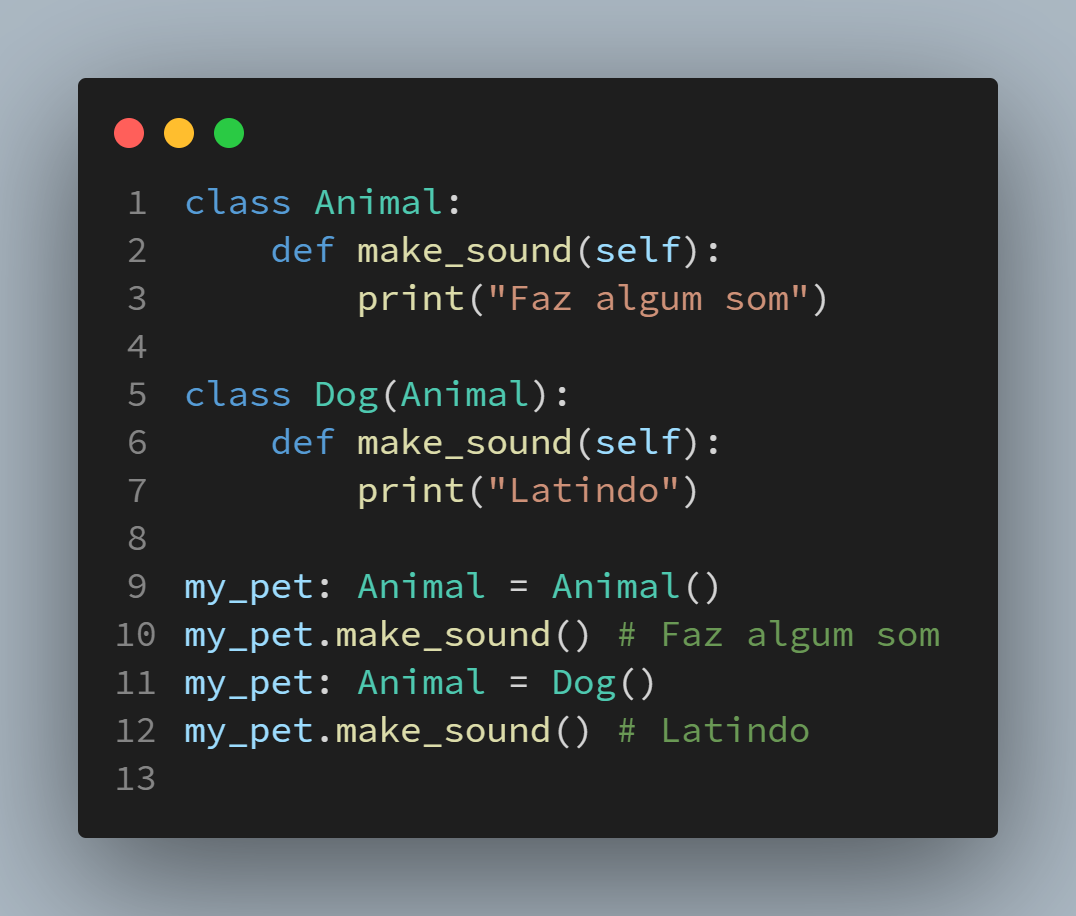
\includegraphics[scale=0.18]{images/l_exemple_good.png}
    \end{figure}
\end{frame}
%% ---------------------------------------------------------------------------

%% ---------------------------------------------------------------------------
\begin{frame}{Interface Segregation}
    \centering
    \textbf{Uma \emph{interface} não deve forçar seus clientes a depender de
    métodos que eles não usam.}
\end{frame}

\begin{frame}{Exemplo \textcolor{gred}{Ruim}}
    \begin{figure}
        \centering
        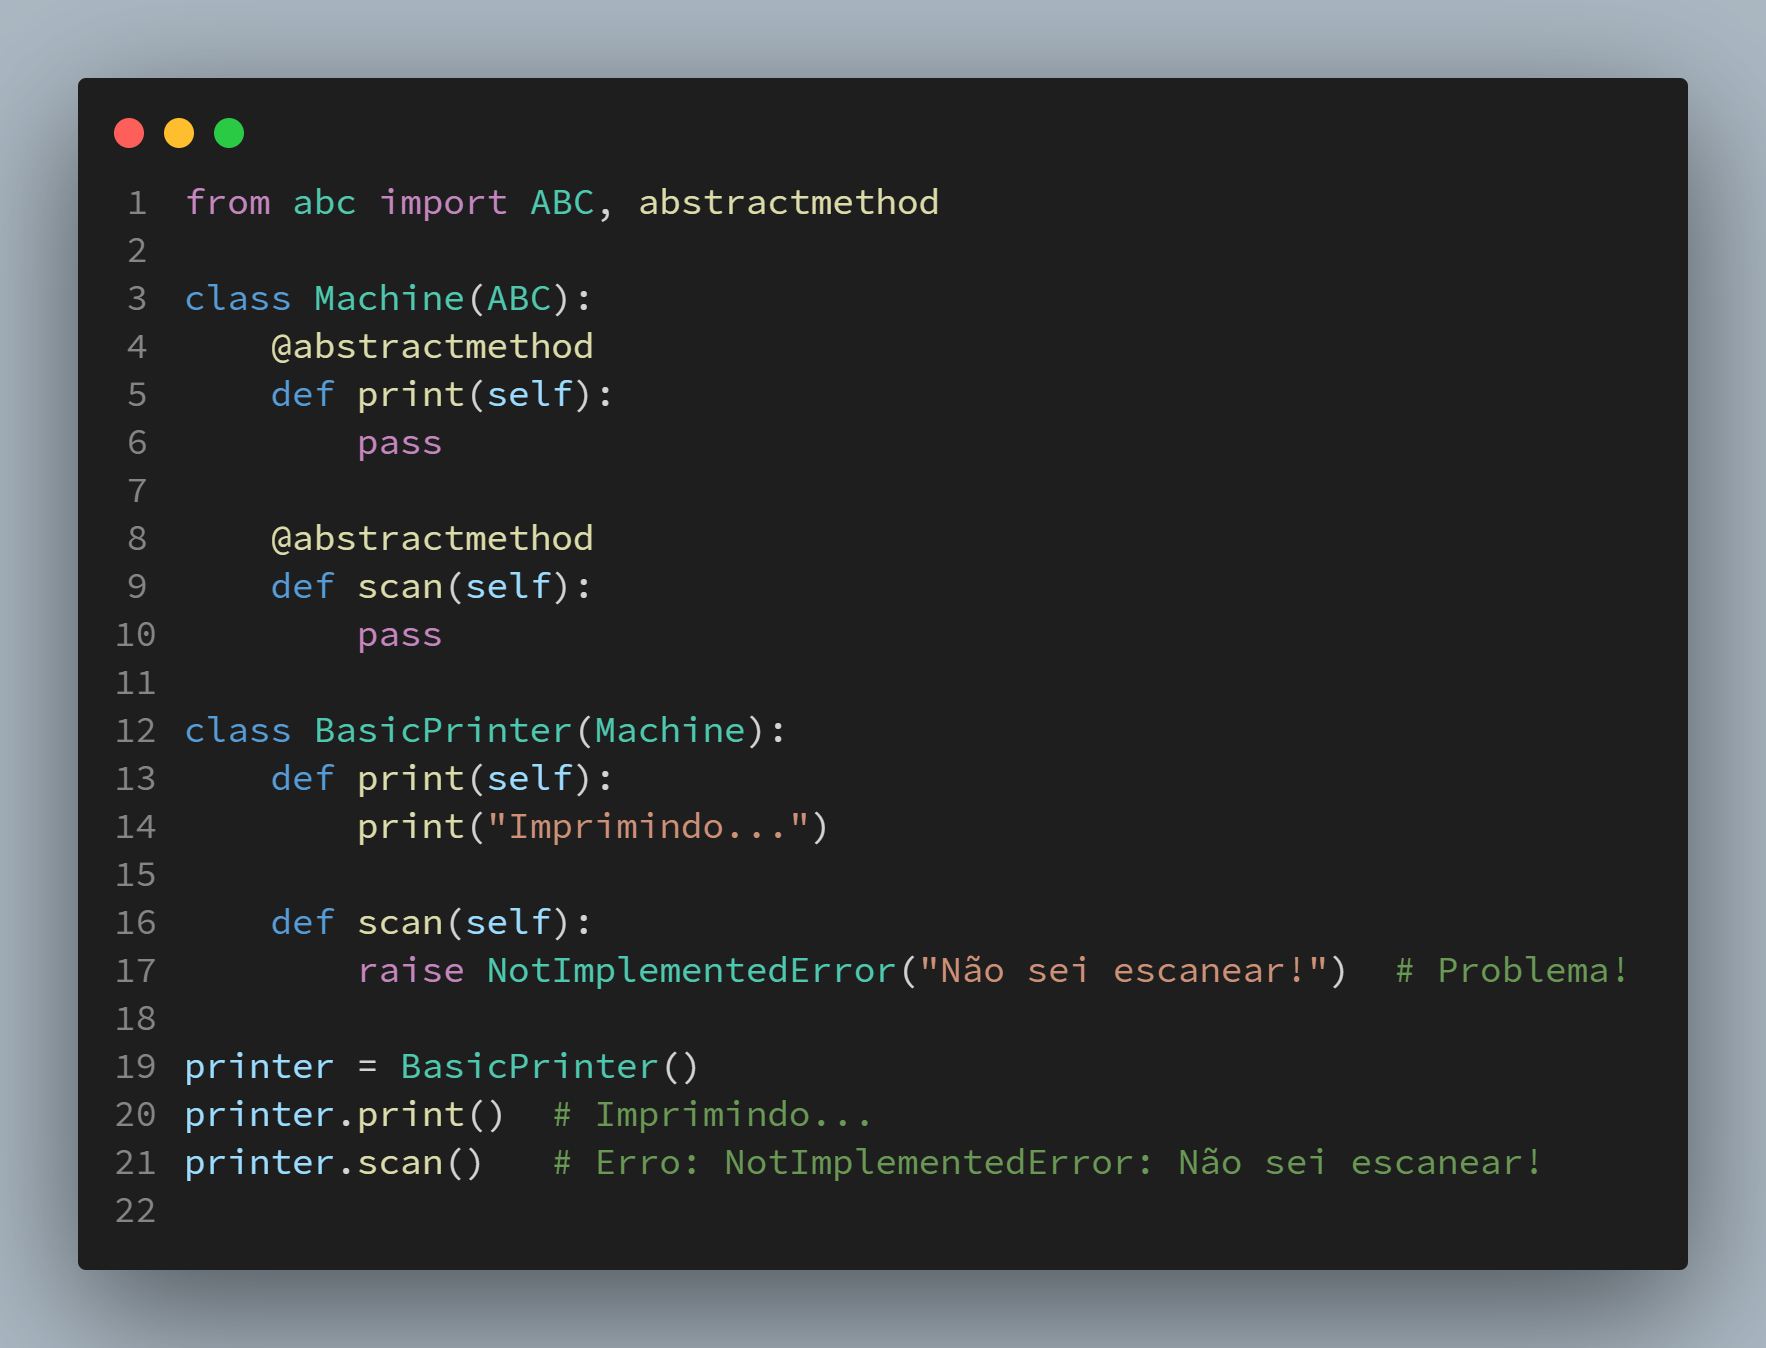
\includegraphics[scale=0.13]{images/i_exemple_bad.png}
    \end{figure}
\end{frame}

\begin{frame}{Exemplo \textcolor{ggreen}{Bom}}
    \begin{figure}
        \centering
        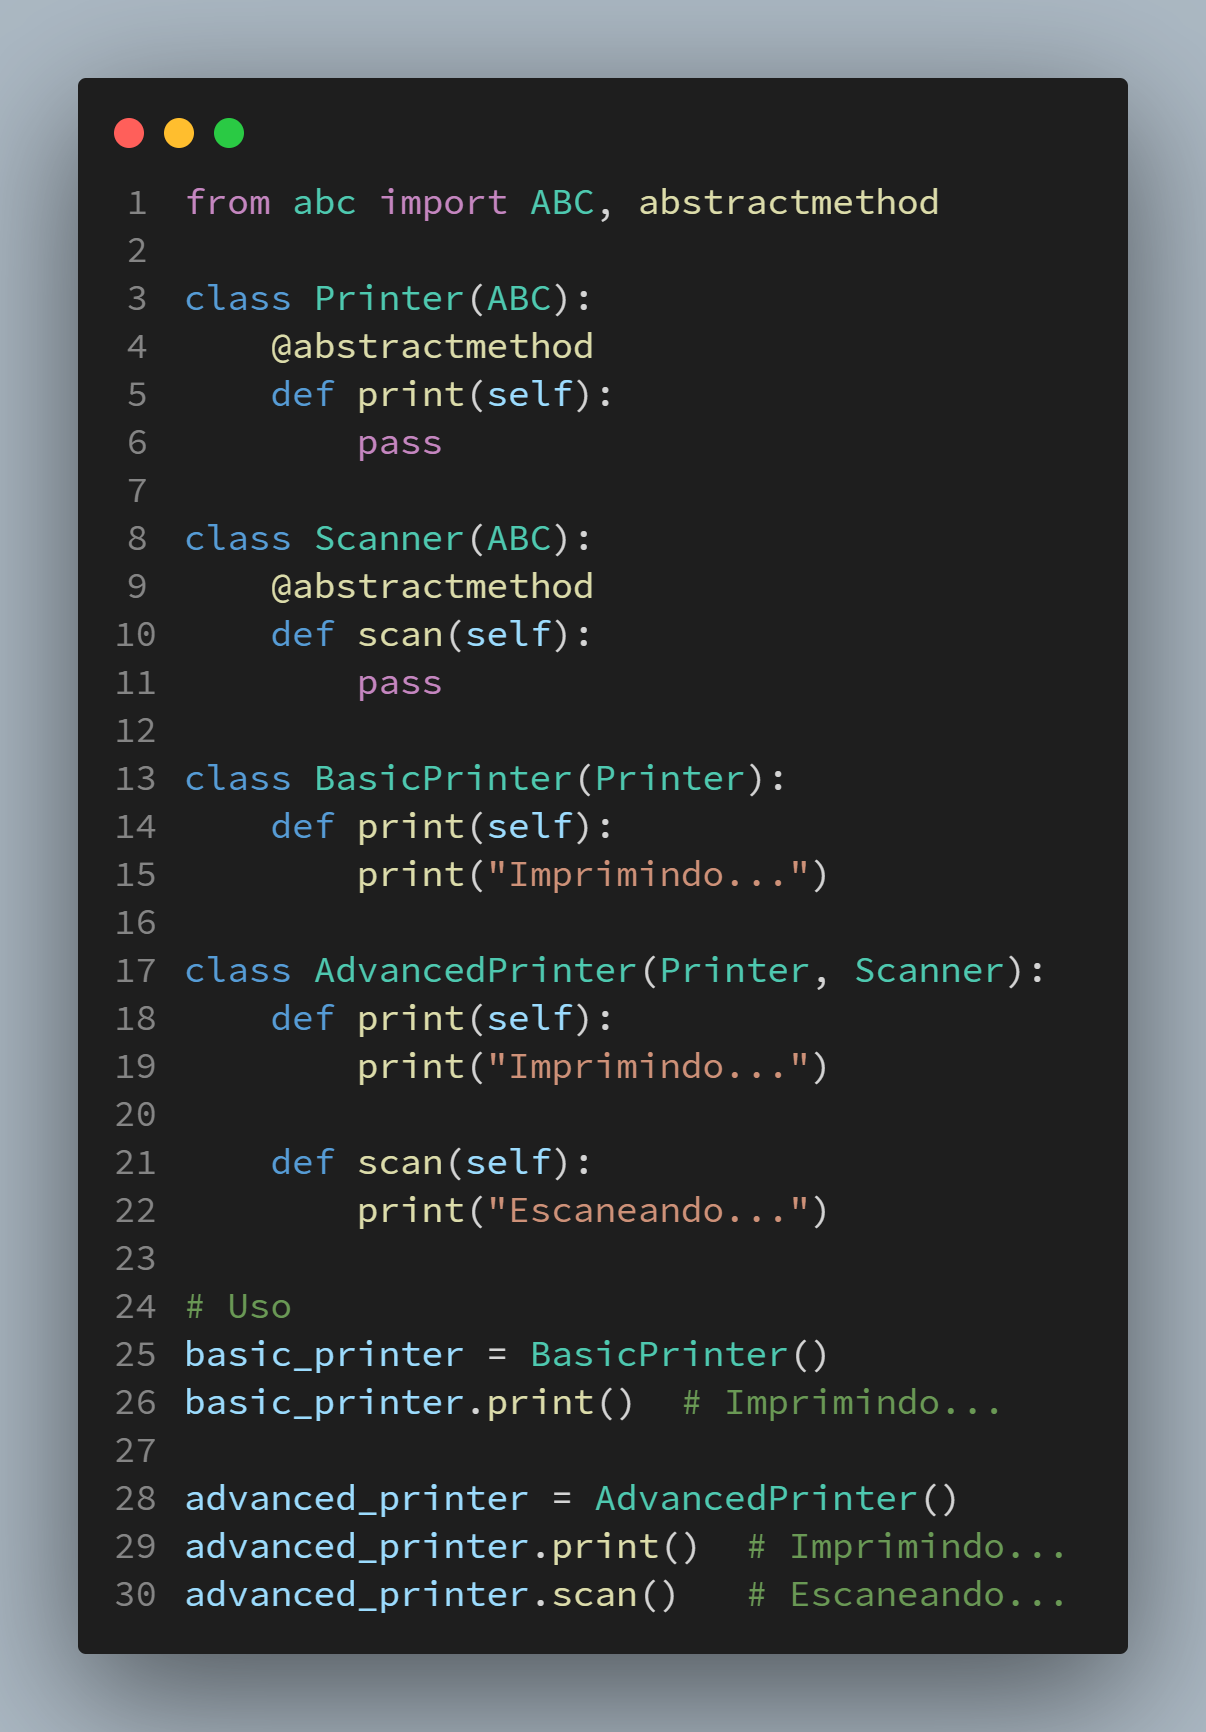
\includegraphics[scale=0.12]{images/i_exemple_good.png}
    \end{figure}
\end{frame}
%% ---------------------------------------------------------------------------

%% ---------------------------------------------------------------------------
\begin{frame}{Dependency Inversion}
    \centering
    \textbf{\emph{Módulos de alto nível} não devem depender de \emph{módulos de
    baixo nível}. Ambos devem depender de \emph{abstrações}.}

    \vspace{20px}

    \textbf{\emph{Abstrações} não devem depender de \emph{detalhes}. Detalhes
    devem depender de \emph{abstrações.}}
\end{frame}

\begin{frame}{Exemplo \textcolor{gred}{Ruim}}
    \begin{figure}
        \centering
        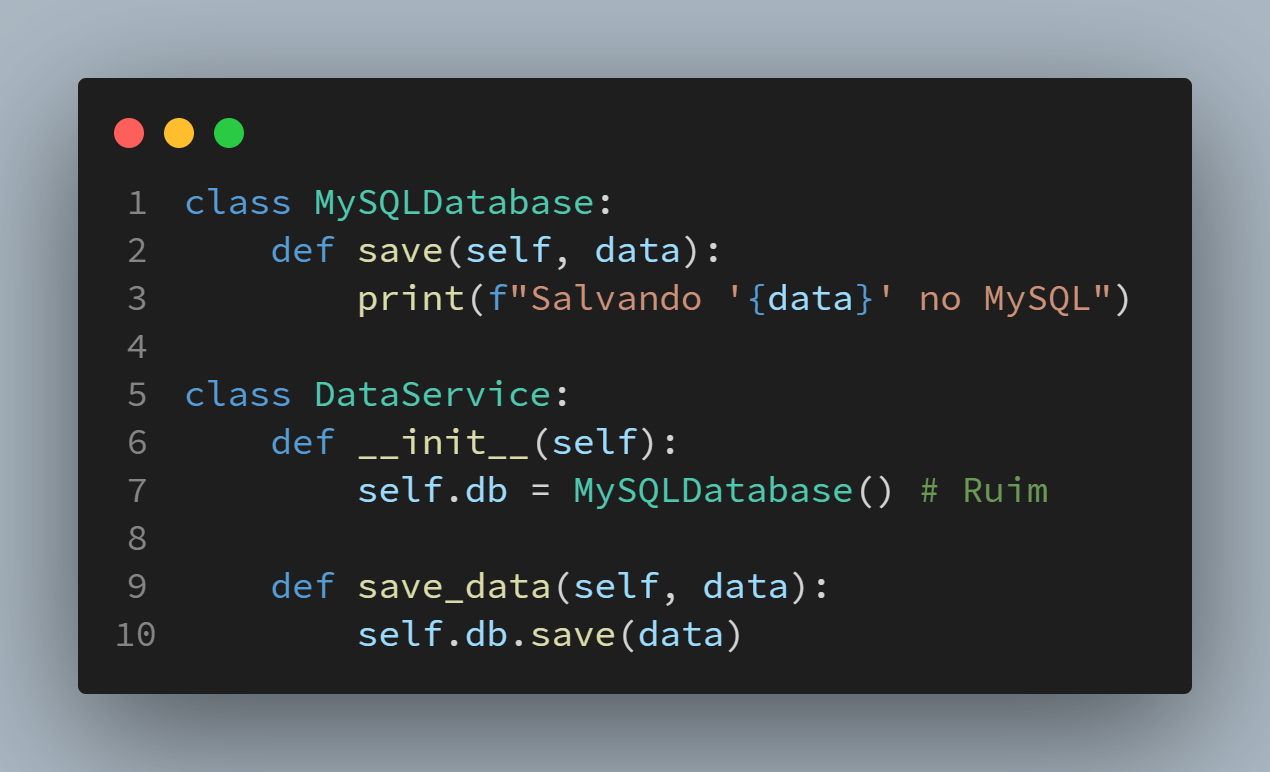
\includegraphics[scale=0.20]{images/d_exemple_bad.png}
    \end{figure}
\end{frame}

\begin{frame}{Exemplo \textcolor{ggreen}{Bom}}
    \begin{figure}
        \centering
        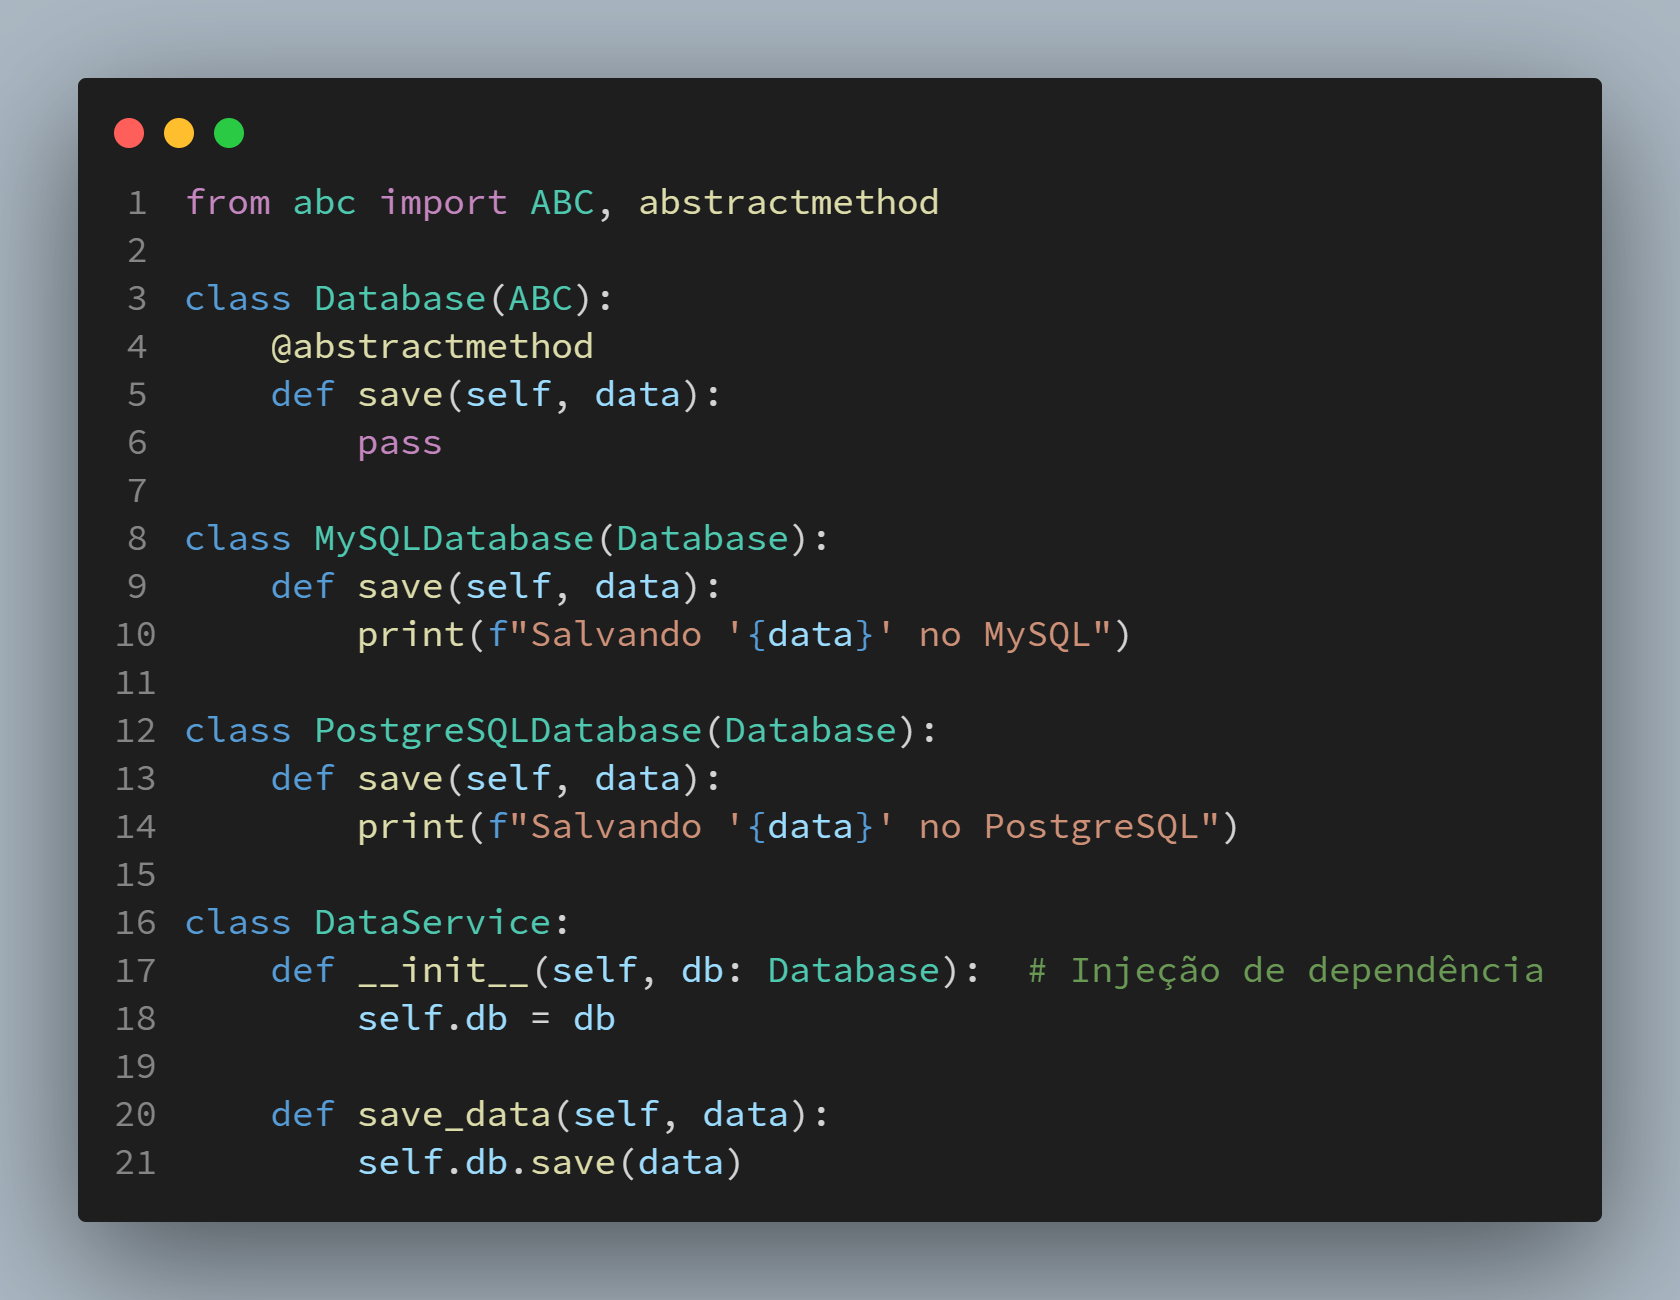
\includegraphics[scale=0.14]{images/d_exemple_good.png}
    \end{figure}
\end{frame}
%% ---------------------------------------------------------------------------

% Final frame
\begin{frame}{}
    \centering
    \huge{\textbf{\example{Obrigado(a) pela Atenção!}}}
\end{frame}

\end{document}